%*****************************************************
%	APPENDIX
%*****************************************************
\appendix
\chapter{Common examples}
\label{ch:appendix}
%-----------------------------------------------------
% Here are some useful LaTEX examples.
% - Block diagrams 
% -	Equations
% - Figures
% - Code
% - Circuit diagrams
% Please note that there often many ways of entering
% this type of information. 
%====================================================
\section{Block Diagrams}
\label{sec:appendix.blockdiagram}
%----------------------------------------------------
%@@@@@@@@@@@@@@@@@@@@@@@@@@@@@
% Simple block (note that 'block' etc. have been defined in thesis.tex
%@@@@@@@@@@@@@@@@@@@@@@@@@@@@@
\begin{figure}[ht]
	\centering
	\begin{tikzpicture}[font=\fontfamily{phv}\selectfont]
		\node[block, align=center]       (a) 	 {Electrical Network};
		\node[left =of a,font=\bfseries] (text1) {Input(s)};
		\node[right=of a,font=\bfseries] (text2) {Output(s)};
		\draw[->] (text1) -- (a);
		\draw[->] (a)     -- (text2);
	\end{tikzpicture}
	\caption{\textbf{A black box}}
   	\label{fig:blackbox}
\end{figure}
%@@@@@@@@@@@@@@@@@@@@@@@@@@@@@

%@@@@@@@@@@@@@@@@@@@@@@@@@@@@@
% Compilation block diagram
%@@@@@@@@@@@@@@@@@@@@@@@@@@@@@
\begin{figure}[ht]
	\centering
\begin{tikzpicture}[auto, node distance=3.5cm,>=latex']

    \node [block2, align=center] 					(block1) 	{\nfont{phv}{Pre-processor}\\
    															(\nfont{pcr}{\small cpp} )};
    \node [block2, right of=block1, align=center] 	(block2) 	{\nfont{phv}{Compiler}\\
    														    (\nfont{pcr}{\small cc1} )};
    \node [block2, right of=block2, align=center] 	(block3) 	{\nfont{phv}{Assembler}\\
    															(\nfont{pcr}{\small as} )};
	\node [block2, right of=block3, align=center] 	(block4) 	{\nfont{phv}{Linker}\\
    														    (\nfont{pcr}{\small ld} )};
	\draw		(-2.5,0)coordinate 		(in);
	\draw		(13,0)coordinate 		(out);
	
	\draw		(-2,0)coordinate 		(A);
	\draw		(13,0)coordinate 		(out);
	\draw		(13,0)coordinate 		(out);
	\draw		(13,0)coordinate 		(out);
	\draw		(13,0)coordinate 		(out);
	
	\draw [->]  (in)     -- node[name=main.i, align=center] {\small \text{main.c}} 	 (block1);
	\draw [->] 	(block1) -- node[name=main.i, align=center] {\small \text{main.i}} 	 (block2);
    \draw [->] 	(block2) -- node[name=main.s, align=center] {\small \text{main.s}} 	 (block3);
    \draw [->] 	(block3) -- node[name=main.o, align=center] {\small \text{main.o}} 	 (block4);
    \draw [->] 	(block4) -- node[name=main,   align=center] {\small \text{main.elf}} (out);
 
;\end{tikzpicture}
		
	\caption{\textbf{A block diagram showing the compilation process.} Adapted from \cite{Bryant2011}.}
   	\label{fig:compilation}
\end{figure}
%@@@@@@@@@@@@@@@@@@@@@@@@@@@@@

%@@@@@@@@@@@@@@@@@@@@@@@@@@@@@
% Sequential block diagram
%@@@@@@@@@@@@@@@@@@@@@@@@@@@@@
\begin{figure}[ht]
	\centering

\begin{tikzpicture}[auto, node distance=3cm,>=latex',font=\fontfamily{phv}\selectfont]
    \node [block, align=left] 							(block1) 	{Combinational circuit to get next state};
    \node [block, above of = block1, align=center] 		(block2) 	{Storage elements};
    \node [block, right    = 3cm of block2, align=left] (block3) 	{Combinational circuit to get outputs};
    \node [output, right of=block3] (output) {};
	
	\draw 		(-1.3,-1)coordinate  		(A);
	\draw 		(-1.3,1)coordinate  		(B);
	\draw 		(2.8,0)coordinate 			(C)--++
		 		(90:3)coordinate 			(D);
	\draw 		(7,3)coordinate  			(E);
				
	\draw		(C) -- (D);
	\draw [->]  (C) -- node[name = in] {} (block1);

    \draw [->] 	(block2) -- node[name=ps, align=center] {PS} (block3);

	\draw [<-]	($(A)!0.333!(B)$)--++(180:1.5)node[left]{Inputs};
	\draw 		($(A)!0.667!(B)$)--++(180:1.5)node[left]{};
	\draw [->]	(E)--++(0:1.5)node[right]{Outputs};
	\draw 		(-2.8,0.333)coordinate 		(O)--++
		 		(90:2.667)coordinate 		(X);
			  
	\draw [->] (X) -- node[name=ps, align=center] {NS} (block2);
;\end{tikzpicture}		
	\caption{\textbf{The block diagram for a sequential circuit.} The storage elements hold the values of the present state of the system. The next state (NS) is determined by a combination of the present state (PS) and the input values; and the system outputs are determined by a combinational circuit which takes the present state of the system as input.}
   	\label{fig:seqblock}
\end{figure}
%@@@@@@@@@@@@@@@@@@@@@@@@@@@@@

%@@@@@@@@@@@@@@@@@@@@@@@@@@@@@
% flow chart
%@@@@@@@@@@@@@@@@@@@@@@@@@@@@@
\begin{figure}[H]
\begin{center}
	\begin{tikzpicture}[node distance=1.5cm,font=\fontfamily{phv}\selectfont]

		\draw (0,1) node[anchor=south,circle,draw]{ };
		\draw (0,-5) node[anchor=north,circle,draw]{ };
	
		\draw (0,1.8)node[]{START};
		\draw (0,-5.8)node[]{END};
		\draw (2,-3)coordinate     		(Z);
		
		\node (statement1) [statement] 			           {Statement 1};
		\node (X)   	   [decision, below of=statement1] {?};			
		\node (statement2) [statement,below of=X] 	       {Statement F};
		\node (statement3) [statement,right of=Z] 	       {Statement T};
		
		\draw 	(0,1)coordinate  		(A);
		\draw 	(0,-5)coordinate     	(B);	
												  
		\draw [arrow] (statement1) -- 	(X);
		\draw [arrow] (X) 		   -- 	(statement2);
		
		\draw (1.5,-1.3)node[]{True};
		\draw (0.5,-2.3)node[]{False};
		
		\draw [arrow] (A) 		   -- (statement1);
		\draw [arrow] (statement2) -- (B);
		\draw 		  (X) 		   -- (3.5,-1.5)coordinate(D);
		\draw [arrow] (D) 		   -- (statement3);
		\draw 		  (statement3) -- (3.5,-4)coordinate  (E);
		\draw [arrow] (E)   	   -- (0,-4)coordinate    (F);
	\end{tikzpicture}
	\end{center}
	\caption{\textbf{A flow diagram of an \nfont{pcr}{if} statement.} The direction of the program flow can be altered using a conditional statement, such as \nfont{pcr}{if}. In this example if the condition is TRUE, statement T will be implemented, while if the the condition is FALSE, statement F will be implemented.}
   	\label{fig:flowchart2}
\end{figure}
%@@@@@@@@@@@@@@@@@@@@@@@@@@@@@

%@@@@@@@@@@@@@@@@@@@@@@@@@@@@@
% ASM chart
%@@@@@@@@@@@@@@@@@@@@@@@@@@@@@
\begin{figure}[H]
\begin{center}
\vskip 0.2cm
	\begin{tikzpicture}[node distance=2.5cm,font=\fontfamily{phv}\selectfont]

		\node (state00) [state] 				 {$LED_{1} = 1$\\
										  		  $LED_{2} = 1$\\
												  $LED_{3} = 1$};
												  
		\draw (-2,-2.5)coordinate  		(A0);
		\draw (-2,1.5)coordinate  		(B0);
		\draw (0,1.5)coordinate 	 	(C0);

		
		\node (arr1)   [decision, below of=state00] {Arr?};
		\node (store1) [condition, below of=arr1]   {Store 1};
		
		\node (state01) [state, below of=store1] {$LED_{1} = 0$\\
										  		  $LED_{2} = 1$\\
												  $LED_{3} = 1$};
												  
		\draw (-2,-10)coordinate  	(A1);
		\draw (-2,-6)coordinate  	(B1);
		\draw (0,-6)coordinate 	 	(C1);

		
		\node (arr2)   [decision, below of=state01] {Arr?};
		\node (store2) [condition, below of=arr2]   {Store 2};												  
			
		\draw (3,0)coordinate  		(11);
		\draw (3,-7.5)coordinate  	(10);	
		
		\node (state11) [state, right of=11] {$LED_{1} = 0$\\
										      $LED_{2} = 0$\\
											  $LED_{3} = 1$};
											  
		\node (arr3)   [decision, below of=state11] {Arr?};
		\node (store3) [condition, below of=arr3]   {Store 3};											  

		\node (state10) [state, right of=10] {$LED_{1} = 0$\\
										      $LED_{2} = 0$\\
											  $LED_{3} = 0$};
											  
											  
		\draw 		(3.5,1.5)coordinate  		(A2);
		\draw 		(3.5,-13.7)coordinate  		(B2);
		\draw		(0,-13.7)coordinate 	 	(C2);
		\draw 		(5.5,1.5)coordinate  		(D2);
			
		\draw 		(7.5,-2.5)coordinate  		(A3);
		\draw 		(7.5,1.5)coordinate  	    (B3);
		\draw		(5.5,1.5)coordinate 	 	(C3);
			
		\draw 		(7.5,-9)coordinate  		(A4);
		\draw 		(7.5,-6)coordinate  		(B4);
		\draw		(5.5,-6)coordinate 	 	    (C4);
		\draw 		(5.5,-9)coordinate  		(D4);							  
										  	
		\draw (A2)         -- (B2);	
		\draw (B2)         -- (C2);	
		\draw (store2)     -- (C2);	
		\draw (A2)         -- (D2);
		\draw [arrow] (D2) -- (state11);
		\draw (arr1)       -- (A0);
		\draw (A0)         -- (B0);
		\draw (B0)         -- (C0);
		\draw [arrow] (C0) -- (state00);
	
		\draw (A1)         -- (B1);	
		\draw [arrow] (B1) -- (C1);
		\draw (arr2)       -- (A1);
		
		\draw (A3)         -- (B3);	
		\draw (B3)         -- (C3);
		\draw (arr3)       -- (A3);
		
		\draw (A4)         -- (B4);	
		\draw [arrow] (B4) -- (C4);
		\draw (A4)         -- (D4);
		\draw (D4) -- (state10);
	
																		  
		\draw [arrow] (state00) -- (arr1);
		\draw [arrow] (arr1)    -- (store1);
		\draw [arrow] (store1)  -- (state01);
		\draw [arrow] (state01) -- (arr2);
		\draw [arrow] (arr2)    -- (store2);
		\draw [arrow] (state11) -- (arr3);
		\draw [arrow] (arr3)    -- (store3);
		\draw [arrow] (store3)  -- (state10);

%
		\draw 	(0.75,1)node[]{00};
		\draw 	(0.75,-6.5)node[]{01};
		\draw 	(6.2,1)node[]{11};
		\draw 	(6.2,-6.5)node[]{10};
		
		\draw 	(-3.5,0)node[]	    {\large{Wait for 1}};
		\draw 	(-3.5,-7.5)node[]	{\large{Wait for 2}};
		\draw 	(9,0)node[]		    {\large{Wait for 3}};
		\draw 	(9,-7.5)node[]	    {\large{Wait}};
%		
		\draw 	(-3.5,0)ellipse		(1.2cm and 0.35cm);
		\draw 	(-3.5,-7.5)ellipse	(1.2cm and 0.35cm);
		\draw 	(9,0)ellipse		(1.2cm and 0.35cm);
		\draw 	(9,-7.5)ellipse	    (1.2cm and 0.35cm);
		
		\draw 	(0.2,-3.5)node[]	    {\large{1}};
		\draw 	(0.2,-11)node[]  	    {\large{1}};
		\draw 	(5.7,-3.5)node[]		{\large{1}};
		\draw 	(-1.2,-2.3)node[]	    {\large{0}};
		\draw 	(-1.2,-9.8)node[]  	    {\large{0}};
		\draw 	(6.7,-2.3)node[]		{\large{0}};

	\end{tikzpicture}
	\end{center}
		\caption{\textbf{An Algorithmic State Machine.} }
   	\label{fig:asm}
\end{figure}

%@@@@@@@@@@@@@@@@@@@@@@@@@@@@@

%----------------------------------------------------
\section{Equations}
\label{sec:appendix.equations}
%----------------------------------------------------
%&&&&&&&&&&&&&&&&&&&&&&&&&&&&&&&&&&&&&&&&&&&&&&
% Basic single line equation 
%&&&&&&&&&&&&&&&&&&&&&&&&&&&&&&&&&&&&&&&&&&&&&&
\begin{equation}
	\centering 
	D = \log_2 N\ \mbox{			[bits]}
	\label{eq:info}
\end{equation}
%&&&&&&&&&&&&&&&&&&&&&&&&&&&&&&&&&&&&&&&&&&&&&&

%&&&&&&&&&&&&&&&&&&&&&&&&&&&&&&&&&&&&&&&&&&&&&&
% Equation with brackets over certain terms
% Note that the * suppresses equation numbers
%&&&&&&&&&&&&&&&&&&&&&&&&&&&&&&&&&&&&&&&&&&&&&&
		\begin{equation*}
			Y = \underbrace{A}_\text{{\color{blue}literal}}\overbrace{\overline{B}}^\text{{\color{blue}complement}}+\overbrace{\overline{A}BC+\underbrace{AC}_\text{{\color{blue}product}}}^\text{{\color{blue}sum}}		
		\label{eq:boolean}
		\end{equation*}
%&&&&&&&&&&&&&&&&&&&&&&&&&&&&&&&&&&&&&&&&&&&&&&

%&&&&&&&&&&&&&&&&&&&&&&&&&&&&&&&&&&&&&&&&&&&&&&
% Equations with multiple lines
% Note that the & is used to hold the position for
% the next line
%&&&&&&&&&&&&&&&&&&&&&&&&&&&&&&&&&&&&&&&&&&&&&&
\begin{equation}
\begin{split}
	B 			 &= B \oplus 0\\
	\overline{B} &= B \oplus 1\\
	\label{eq:truefalse}
\end{split}
\end{equation}	
%&&&&&&&&&&&&&&&&&&&&&&&&&&&&&&&&&&&&&&&&&&&&&&

%&&&&&&&&&&&&&&&&&&&&&&&&&&&&&&&&&&&&&&&&&&&&&&
% Equations with different cases
%&&&&&&&&&&&&&&&&&&&&&&&&&&&&&&&&&&&&&&&&&&&&&&
\begin{equation}
		\text{equality}=
		\begin{cases}
			0, & (A \ne B) \\
			1, & (A == B) \\	
		\end{cases}
		\label{eq:equality}
\end{equation}	
%&&&&&&&&&&&&&&&&&&&&&&&&&&&&&&&&&&&&&&&&&&&&&&
%----------------------------------------------------
\section{Figures and tables}
\label{sec:appendix.fig}
%----------------------------------------------------

%@@@@@@@@@@@@@@@@@@@@@@@@@@@@@
% Combining a table and figure into a single figure
% with sub-captions
%@@@@@@@@@@@@@@@@@@@@@@@@@@@@@
\begin{figure}[ht]
	\begin{subfigure}[b]{.45\linewidth}
   		\centering
  		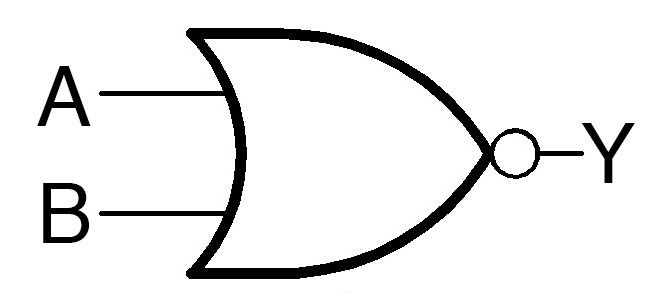
\includegraphics[scale = 1]{figs/nor}
   		\caption{NOR gate symbol}
   		\label{fig:norsym}
 	\end{subfigure}
 \quad
	 \begin{subtable}[b]{.45\linewidth}
   		\centering
   		\begin{tabular}{c c | c}
			\hline\hline
			\multicolumn{2}{c}{\bfseries Input} & \bfseries Output\\
			\hline
		 	A & B &  Y\\
			\hline
			0 & 0 & 1\\
			0 & 1 & 0\\
			1 & 0 & 0\\
			1 & 1 & 0\\
			\hline
		\end{tabular}
		\caption{NOR gate truth table}
		\label{table:nortruth}
	\end{subtable}
  	\caption{\bfseries The NOR gate}
	\label{fig:norgate}
 \end{figure}
 %@@@@@@@@@@@@@@@@@@@@@@@@@@@@@

%@@@@@@@@@@@@@@@@@@@@@@@@@@@@@
% including a picture
\begin{figure}[ht]
  	\centering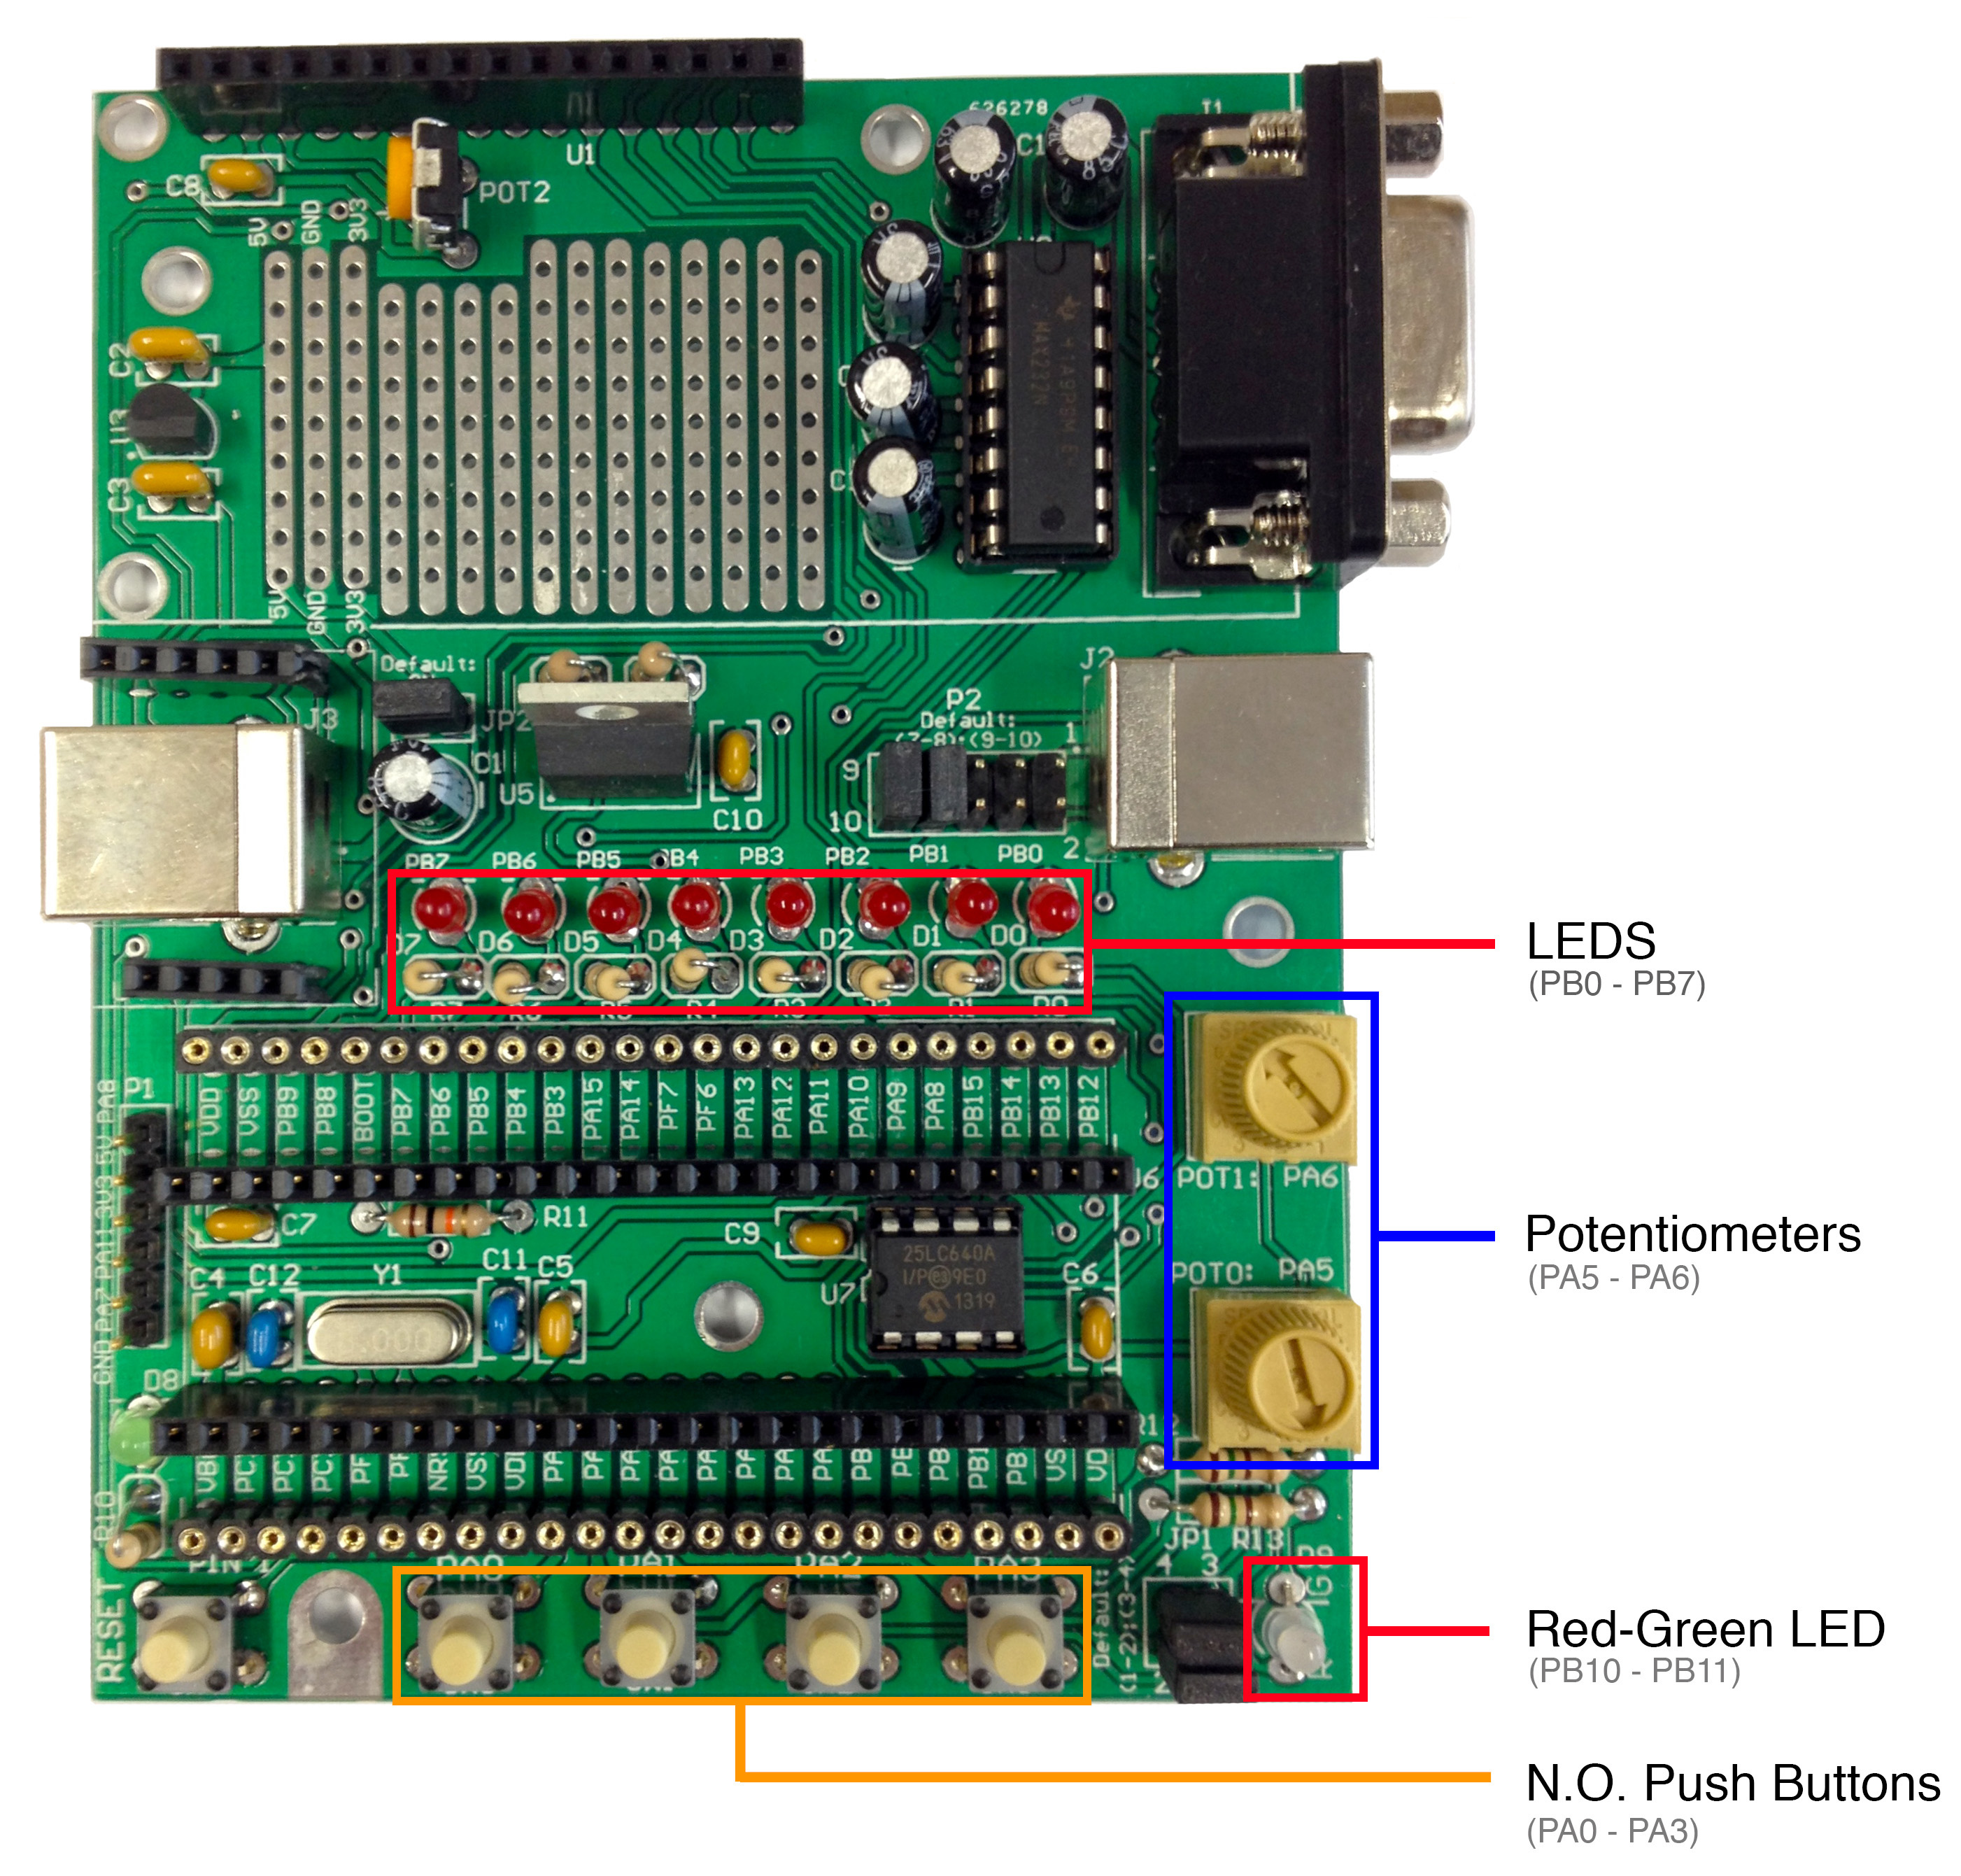
\includegraphics[scale = 0.1]{figs/STM32F0io}
	
	\caption{{\bfseries The simple input/output devices on the UCT STM32F0 development board.} The basic I/O devices on the development board have been labelled as follows: {\color{red}red} - digital outputs which have been connected to LEDS, {\color{YellowOrange} orange} - digital inputs which have been connected to normally open push buttons and {\color{blue} blue} - analogue inputs connected to two potentiometers.}
	\label {fig:STM32F0io}
\end{figure}
%@@@@@@@@@@@@@@@@@@@@@@@@@@@@@
\pagebreak
%----------------------------------------------------
\section{Code}
\label{sec:appendix.code}
%----------------------------------------------------
\begin{Verbatim}[fontfamily=courier,fontsize=\small, numbers=left,commandchars=\\\{\}]
\textcolor{Green}{//*************************************************}
\textcolor{Green}{//* EEE3017W STM32F0                              *}
\textcolor{Green}{//* LCD MODULE LIBRARY                            *}
\textcolor{Green}{//=================================================}
\textcolor{Green}{//* WRITTEN BY:   Samuel Ginsberg                 *}
\textcolor{Green}{//* PORTED BY:    James Gowans                    *}
\textcolor{Green}{//* MODIFIED BY:  Robyn Verrinder                 *}
\textcolor{Green}{//* DATE CREATED: 2004                            *}
\textcolor{Green}{//* PORTED:       2014                            *}                         
\textcolor{Green}{//* MODIFIED:     03-08-2015                      *}
\textcolor{Green}{//=================================================}
\textcolor{Green}{//* PROGRAMMED IN: ECLIPSE IDE Luna  (4.4.1)      *}
\textcolor{Green}{//* DEV. BOARD:    UCT STM32 Development Board    *}
\textcolor{Green}{//=================================================}
\textcolor{Green}{//* DESCRIPTION:   This code contains common      *}
\textcolor{Green}{//*                functions to communicate       *}
\textcolor{Green}{//*                with the LCD module connected  *}
\textcolor{Green}{//*                to the GT16 uC.                *}
\textcolor{Green}{//=================================================}
\textcolor{Green}{//* LCD SETUP:     - 4 bit mode                   *}
\textcolor{Green}{//*                (Upper 4 data lines D4-D7 used)*}
\textcolor{Green}{//*                - Two lines used               *}
\textcolor{Green}{//*                - Flashing cursor              *}
\textcolor{Green}{//=================================================}
\textcolor{Green}{//* CONNECTIONS:                                  *}
\textcolor{Green}{//-------------------------------------------------}
\textcolor{Green}{//* PINS |NAME                     |CONNECTED TO  *}
\textcolor{Green}{//-------------------------------------------------}
\textcolor{Green}{//* 1.....VSS.......................GND           *}
\textcolor{Green}{//* 2.....VDD.......................+5V           *}
\textcolor{Green}{//* 3.....CONTRAST..................POT 2         *}
\textcolor{Green}{//* 4.....RS  - Register Select.....PC14 (LCD_RS) *}
\textcolor{Green}{//* 5.....RW  - Read/Write..........GND           *}
\textcolor{Green}{//* 6.....E   - Enable..............PC15 (LCD_E)  *}
\textcolor{Green}{//* 7.....D0  - Data line 0.........GND           *}
\textcolor{Green}{//* 8.....D1  - Data line 1.........GND           *}
\textcolor{Green}{//* 9.....D2  - Data line 2.........GND           *}
\textcolor{Green}{//* 10....D3  - Data line 3.........GND           *}
\textcolor{Green}{//* 11....D4  - Data line 4.........PB8  (LCD_D4) *}
\textcolor{Green}{//* 12....D5  - Data line 5.........PB9  (LCD_D5) *}
\textcolor{Green}{//* 13....D6  - Data line 6.........PA12 (LCD_D6) *}
\textcolor{Green}{//* 14....D7  - Data line 7.........PA15 (LCD_D7) *}
\textcolor{Green}{//* 15....CATHLED...................NC            *}
\textcolor{Green}{//* 16....ANODELED..................NC            *}
\textcolor{Green}{//*************************************************}
\textcolor{Green}{// INCLUDE FILES}
\textcolor{Green}{//=================================================}
\textcolor{purple}{#include} \textcolor{blue}{"lcd_stm32f0.h"}   
\textcolor{purple}{#include} \textcolor{blue}{"stm32f0xx.h"} 
\textcolor{Green}{//=================================================}
\textcolor{Green}{// SEND COMMAND CODE TO LCD - LCD_Command(command)}
\textcolor{Green}{//=================================================}
\textcolor{Green}{// DESCRIPTION: This function sends a command to }
\textcolor{Green}{//              the LCD. Care is taken not to }
\textcolor{Green}{//              interfere with the other lines }
\textcolor{Green}{//              on the port.  As we are using a}
\textcolor{Green}{//              microcontroller to control the LCD}
\textcolor{Green}{//              we use 4-bit mode to save on number}
\textcolor{Green}{//              of lines used to connect to the LCD. }
\textcolor{Green}{//              This means that an 8-bit command}
\textcolor{Green}{//              must be split into two sets }
\textcolor{Green}{//              of 4-bits (upper and lower)}
\textcolor{Green}{//              These sets must be transmitted}
\textcolor{Green}{//=================================================}
\textcolor{Green}{// USEFUL COMMANDS:}
\textcolor{Green}{// - POWER_UP:      Power up initialization for the lcd}
\textcolor{Green}{// - FOURBIT_MODE:  Sets LCD for 4-bit mode}
\textcolor{Green}{// - TWOLINE_MODE:  Sets up 2 lines and character size}
\textcolor{Green}{// - SETUP_CURSOR:  Turn display on and set up cursor}
\textcolor{Green}{// - CLEAR:         Clear screen}
\textcolor{Green}{// - CURSOR_HOME:   Cursor home}
\textcolor{Green}{// - LINE_TWO:      Line 2}
\textcolor{Green}{//=================================================}
\textcolor{blue}{void} lcd_command(\textcolor{blue}{unsigned char} command)
\{
	\textcolor{Green}{// Register Select (RS)line low} 
	\textcolor{Green}{//(data sent will now be read as commands)}
	GPIOC->BSRR |= LCD_RS_RESET;
    			  
	\textcolor{Green}{// Put upper nibble (upper 4-bits) on data lines, command mode}
	\textcolor{Green}{// DATALINE 7}
	\textcolor{Green}{// Select bit 7 of command, if HIGH set Data line 7 (D7) }
	\textcolor{Green}{// else RESET D7}
	\textcolor{blue}{if} ((command & 0x80) != \textcolor{blue}{0}) 				     
	\{
		GPIOA->BSRR |= LCD_D7_SET;
	\}
	\textcolor{blue}{else}
	\{
		GPIOA->BSRR |= LCD_D7_RESET;
	\}
    
	\textcolor{Green}{// DATALINE 6}
	\textcolor{Green}{// Select bit 6 of command, if HIGH set Data line 6 (D6)}
	\textcolor{Green}{// else RESET D6}
	\textcolor{blue}{if} ((command & 0x40) != \textcolor{blue}{0})			    
	\{
		GPIOA->BSRR |= LCD_D6_SET;
	\}
	\textcolor{blue}{else}
	\{
		GPIOA->BSRR |= LCD_D6_RESET;
	\}
    
	\textcolor{Green}{// DATALINE 5}
	\textcolor{Green}{// Select bit 5 of command, if HIGH set Data line 5 (D5) }
	\textcolor{Green}{// else RESET D5}
	\textcolor{blue}{if} ((command & 0x20) != \textcolor{blue}{0})
	\{
		GPIOB->BSRR |= LCD_D5_SET;             
	\}
	\textcolor{blue}{else}
	\{
		GPIOB->BSRR |= LCD_D5_RESET;
	\}
    
	\textcolor{Green}{// DATALINE 4}
	\textcolor{Green}{// Select bit 4 of command, if HIGH set Data line 4 (D4)} 
	\textcolor{Green}{// else RESET D4}
	\textcolor{blue}{if} ((command & 0x10) != \textcolor{blue}{0})		      
	\{
		GPIOB->BSRR |= LCD_D4_SET;
	\}
	\textcolor{blue}{else}
	\{
		GPIOB->BSRR |= LCD_D4_RESET;
	\}
	
	\textcolor{Green}{// Send data}
	pulse_strobe ();					   

	\textcolor{Green}{// lower nibble to data lines}
	\textcolor{Green}{// Select bit 3 of command, if HIGH set Data line 7 (D7)} 
	\textcolor{Green}{// else RESET D7}
	\textcolor{blue}{if} ((command & 0x08) != \textcolor{blue}{0}) 			       
	\{
		GPIOA->BSRR |= LCD_D7_SET;
	\}
	\textcolor{blue}{else}
	\{
		GPIOA->BSRR |= LCD_D7_RESET;
	\}
    
	\textcolor{Green}{// DATALINE 6}
	\textcolor{Green}{// Select bit 2 of command, if HIGH set Data line 6 (D6)} 
	\textcolor{Green}{// else RESET D6}
	\textcolor{blue}{if} ((command & 0x04) != \textcolor{blue}{0})			    
	\{
		GPIOA->BSRR |= LCD_D6_SET;
	\}
	\textcolor{blue}{else}
	\{
		GPIOA->BSRR |= LCD_D6_RESET;
	\}
    
	\textcolor{Green}{// DATALINE 5}
	\textcolor{Green}{// Select bit 1 of command, if HIGH set Data line 5 (D5)}
	\textcolor{Green}{// else RESET D5}
	\textcolor{blue}{if} ((command & 0x02) != \textcolor{blue}{0})
	\{
		GPIOB->BSRR |= LCD_D5_SET;             
	\}
	\textcolor{blue}{else}
	\{
		GPIOB->BSRR |= LCD_D5_RESET;
	\}
    
	\textcolor{Green}{// DATALINE 4}
	\textcolor{Green}{// Select bit 0 of command, if HIGH set Data line 5 (D5)}
	\textcolor{Green}{// else RESET D5}
	\textcolor{blue}{if} ((command & 0x01) != \textcolor{blue}{0})		       
	\{
		GPIOB->BSRR |= LCD_D4_SET;
	\}
	\textcolor{blue}{else}
	\{
		GPIOB->BSRR |= LCD_D4_RESET;
	\}
    
	\textcolor{Green}{// Send data}
	pulse_strobe();                          
	delay(\textcolor{blue}{3000});
\}
\textcolor{Green}{//=================================================}
\textcolor{Green}{// INITIALISE LCD - LCD_Init()}
\textcolor{Green}{//=================================================}
\textcolor{Green}{// DESCRIPTION: This function sets up the port }
\textcolor{Green}{//              lines for the LCD and}
\textcolor{Green}{//              intialises the module for use.}
\textcolor{Green}{//=================================================}
\textcolor{Green}{// LCD SETUP:     - 4 bit mode      }
\textcolor{Green}{//                 (Upper 4 data lines D4-D7 used)}
\textcolor{Green}{//                - Two lines used}
\textcolor{Green}{//                - Flashing cursor}
\textcolor{Green}{//=================================================}
\textcolor{blue}{void} init_LCD(\textcolor{blue}{void})
\{
	\textcolor{Green}{// Connect clocks to GPIO A, B and C}
	RCC->AHBENR |= RCC_AHBENR_GPIOAEN; 		  
	RCC->AHBENR |= RCC_AHBENR_GPIOBEN;
	RCC->AHBENR |= RCC_AHBENR_GPIOCEN;

	\textcolor{Green}{// D6 and D7}
	GPIOA->MODER |= (GPIO_MODER_MODER12_0|GPIO_MODER_MODER15_0); 
	\textcolor{Green}{// D4 and D5}
	GPIOB->MODER |= (GPIO_MODER_MODER8_0|GPIO_MODER_MODER9_0);   
	\textcolor{Green}{// RS and EN}
	GPIOC->MODER |= (GPIO_MODER_MODER14_0|GPIO_MODER_MODER15_0); 

	\textcolor{Green}{// Allow the LCD some power up time (~30ms)}
	delay(\textcolor{blue}{30000});							  

	\textcolor{Green}{// Power up initialization for the lcd}
	lcd_command(POWER_UP);                    
	\textcolor{Green}{// Set LCD into 4 bit mode}
	lcd_command(FOURBIT_MODE);                
	\textcolor{Green}{// Turn display on and set up cursor}
	lcd_command(DISPLAY_ON);                  
	\textcolor{Green}{// Set up 2 lines and character size}
	lcd_command(TWOLINE_MODE);                
	\textcolor{Green}{// Clear display}
	lcd_command(CLEAR);                       
\}
\textcolor{Green}{//=================================================}
\textcolor{Green}{// WRITE A SINGLE CHARACTER TO THE LCD - LCD_PutChar(character)}
\textcolor{Green}{//=================================================}
\textcolor{Green}{// DESCRIPTION: Puts a single character on the LCD }
\textcolor{Green}{//              at the next position on the screen. }
\textcolor{Green}{//              The character to be printed is in the input}
\textcolor{Green}{//              parameter. For numbers, letters and}
\textcolor{Green}{//              other common characters the ASCII code }
\textcolor{Green}{//              will produce correct display.}
\textcolor{Green}{//               }
\textcolor{Green}{//              Refer to the Hitachi HD44780 datasheet }
\textcolor{Green}{//              for full character set information.}
\textcolor{Green}{//=================================================}
\textcolor{blue}{void} lcd_putchar(\textcolor{blue}{unsigned char} character)
\{
	\textcolor{Green}{// Register Select (RS) line HIGH} 
	\textcolor{Green}{//(data sent will now be read as text)}
	GPIOC->BSRR |= LCD_RS_SET;			  
	    
	\textcolor{Green}{// Put upper nibble (upper 4-bits) on data lines, command mode} 
	\textcolor{Green}{// DATALINE 7}
	\textcolor{Green}{// Select bit 7 of command, if HIGH set Data line 7 (D7)}
	\textcolor{Green}{// else RESET D7}
	\textcolor{blue}{if} ((character & 0x80) != \textcolor{blue}{0}) 				         
	\{
		GPIOA->BSRR |= LCD_D7_SET;
	\}
	\textcolor{blue}{else}
	\{
		GPIOA->BSRR |= LCD_D7_RESET;
	\}

	\textcolor{Green}{// DATALINE 6}
	\textcolor{Green}{// Select bit 6 of command, if HIGH set Data line 6 (D6)}
	\textcolor{Green}{// else RESET D6}
	\textcolor{blue}{if} ((character & 0x40) != \textcolor{blue}{0})			
	\{
		GPIOA->BSRR |= LCD_D6_SET;
	\}
	\textcolor{blue}{else}
	\{
		GPIOA->BSRR |= LCD_D6_RESET;
	\}

	\textcolor{Green}{// DATALINE 5}
	\textcolor{Green}{// Select bit 5 of command, if HIGH set Data line 5 (D5)} 
	\textcolor{Green}{//else RESET D5}
	\textcolor{blue}{if} ((character & 0x20) != \textcolor{blue}{0})
	\{
		GPIOB->BSRR |= LCD_D5_SET;  
	\}
	\textcolor{blue}{else}
	\{
		GPIOB->BSRR |= LCD_D5_RESET;
	\}
        
	\textcolor{Green}{// DATALINE 4}
	\textcolor{Green}{// Select bit 4 of command, if HIGH set Data line 4 (D4)} 
	\textcolor{Green}{//else RESET D4}
	\textcolor{blue}{if} ((character & 0x10) != \textcolor{blue}{0})		          
	\{
		GPIOB->BSRR |= LCD_D4_SET;
	\}
	\textcolor{blue}{else}
	\{
		GPIOB->BSRR |= LCD_D4_RESET;
	\}

	\textcolor{Green}{// Send data}
	pulse_strobe ();					   

	\textcolor{Green}{// lower nibble to data lines}
	\textcolor{Green}{// Select bit 3 of command, if HIGH set Data line 7 (D7)}
	\textcolor{Green}{// else RESET D7}
	\textcolor{blue}{if} ((character & 0x08) != \textcolor{blue}{0}) 			   
	\{
		GPIOA->BSRR |= LCD_D7_SET;
	\}
	\textcolor{blue}{else}
	\{
		GPIOA->BSRR |= LCD_D7_RESET;
	\}
       
	\textcolor{Green}{// DATALINE 6}
	\textcolor{Green}{// Select bit 2 of command, if HIGH set Data line 6 (D6)}
	\textcolor{Green}{// else RESET D6}
	\textcolor{blue}{if} ((character & 0x04) != \textcolor{blue}{0})			
	\{
		GPIOA->BSRR |= LCD_D6_SET;
	\}
	\textcolor{blue}{else}
	\{
		GPIOA->BSRR |= LCD_D6_RESET;
	\}

	\textcolor{Green}{// DATALINE 5}
	\textcolor{Green}{// Select bit 1 of command, if HIGH set Data line 5 (D5)}
	\textcolor{Green}{// else RESET D5}
	\textcolor{blue}{if} ((character & 0x02) != \textcolor{blue}{0})
	\{
		GPIOB->BSRR |= LCD_D5_SET;                 
	\}
	\textcolor{blue}{else}
	\{
		GPIOB->BSRR |= LCD_D5_RESET;
	\}
        
	\textcolor{Green}{// DATALINE 4}
	\textcolor{Green}{// Select bit 0 of command, if HIGH set Data line 5 (D5) }
	\textcolor{Green}{//else RESET D5}
	\textcolor{blue}{if} ((character & 0x01) != \textcolor{blue}{0})		           
	\{
		GPIOB->BSRR |= LCD_D4_SET;
	\}
	\textcolor{blue}{else}
	\{
		GPIOB->BSRR |= LCD_D4_RESET;
	\}       
	\textcolor{Green}{// Send data}
	pulse_strobe();                          
\}
\textcolor{Green}{//=================================================}
\textcolor{Green}{// WRITE A STRING TO THE LCD - LCD_PutString(ptr_String)}
\textcolor{Green}{//=================================================}
\textcolor{Green}{// DESCRIPTION: Writes a string to the LCD. }
\textcolor{Green}{//=================================================}
\textcolor{blue}{void} lcd_putstring(\textcolor{blue}{unsigned char}* instring)           
\{
	\textcolor{blue}{unsigned char} count = \textcolor{blue}{0};
	\textcolor{Green}{// Until the null terminator is reached}
	\textcolor{blue}{while} (instring[count]) 
	\{
		\textcolor{Green}{// Write each character to LCD}
		lcd_putchar(instring[count]);         
		count++;
	\}                             
\}
\textcolor{Green}{//=================================================}
\textcolor{Green}{// PULSE STROBE - Pulse_Strobe()}
\textcolor{Green}{//=================================================}
\textcolor{Green}{// DESCRIPTION: Pulse the strobe line of the LCD }
\textcolor{Green}{//              to indicate that data is ready.}
\textcolor{Green}{//=================================================}
\textcolor{blue}{void} pulse_strobe(\textcolor{blue}{void})
\{
	\textcolor{Green}{// Delay}
	delay(\textcolor{blue}{20});                                  
	\textcolor{Green}{// pull E (PC15) HIGH}
	GPIOC->BSRR |= LCD_EN_SET;			      
	\textcolor{Green}{// Delay}
	delay(\textcolor{blue}{20});                                  
	\textcolor{Green}{// Take EN LOW}
	GPIOC->BSRR |= LCD_EN_RESET;             
	\textcolor{Green}{// Delay}
	delay(\textcolor{blue}{20});                                 
	\textcolor{Green}{// Take EN HIGH}
	GPIOC->BSRR |= LCD_EN_SET;                
\}
\textcolor{Green}{//=================================================}
\textcolor{Green}{// DELAY FUNCTION  - delay()}
\textcolor{Green}{//=================================================}
\textcolor{Green}{// DESCRIPTION: A delay used by the LCD functions. }
\textcolor{Green}{//=================================================}
\textcolor{blue}{void} delay(\textcolor{blue}{void})           
\{
	\textcolor{blue}{volatile unsigned int} counter;
	microseconds *= \textcolor{blue}{3};
	\textcolor{blue}{for}(counter = \textcolor{blue}{0}; counter<microseconds; counter++)
	\{
		__asm(\textcolor{red}{"nop"});
		__asm(\textcolor{red}{"nop"});
	\}                               
\}
\textcolor{Green}{//*************************************************}
\textcolor{Green}{//*               END OF PROGRAM                  *}
\textcolor{Green}{//*************************************************}		
\end{Verbatim}
%----------------------------------------------------
\section{Circuit Diagrams}
\label{sec:appendix.circuits}
%----------------------------------------------------

%@@@@@@@@@@@@@@@@@@@@@@@@@@@@@
% NOR gate = OR + NOT
%@@@@@@@@@@@@@@@@@@@@@@@@@@@@@
\begin{figure}[ht]	
	\centering\begin{circuitikz} [font=\fontfamily{phv}\selectfont]
	\draw
		(0,0) node[or port] (myor) {}
		(1,0) node[not port] (mynot) {}
		(myor.out) -- (mynot.in)
		(myor.in 1) node[anchor=east] {A}
		(myor.in 2) node[anchor=east] {B}
		(mynot.out) node[anchor=west] {Y};
	\end{circuitikz}
 	\caption{{\bfseries The NOR gate.} This gate is made up of an OR gate followed by a NOT gate.}
	\label{fig:notor}
 \end{figure}
%@@@@@@@@@@@@@@@@@@@@@@@@@@@@@

%@@@@@@@@@@@@@@@@@@@@@@@@@@@@@
% Multi-circuit figure
%@@@@@@@@@@@@@@@@@@@@@@@@@@@@@
\begin{figure}[ht]
	\begin{subfigure}[b]{.4\linewidth}
   		\centering
%-----------------------------
% Logic cct 1
%-----------------------------
		\begin{center}
			\begin{circuitikz}[font=\fontfamily{phv}\selectfont]
			\draw
				(1,0.5) 	node[scale=0.6,not port] 	(mynot1) {}
				(1,-0.5) 	node[scale=0.6,not port] 	(mynot2) {}
    			(0,0.5) 	node[anchor=east] {A} -- 	(mynot1.in)
				(0,-0.5) 	node[anchor=east] {B} -- 	(mynot2.in) 
 				(3,0) 		node[and port] 				(myand) {}
       			(mynot1.out) |- 						(myand.in 1)
				(mynot2.out) |- 						(myand.in 2)
				(myand.out) -- (3.5,0) node[anchor=west] {Y}
			;\end{circuitikz}
		\end{center}
%-----------------------------
% Logic cct 2
%-----------------------------
		\begin{center}
			\begin{circuitikz}[font=\fontfamily{phv}\selectfont]
			\draw
				(1,0.5) 	node[scale=0.6,not port] 	(mynot1) {}
				(1,-0.5) 	node[scale=0.6,not port] 	(mynot2) {}
    			(0,0.5) 	node[anchor=east] {A} -- 	(mynot1.in)
				(0,-0.5) 	node[anchor=east] {B} -- 	(mynot2.in) 
 				(3,0) 		node[or port] 				(myor) {}
       			(mynot1.out) |- 						(myor.in 1)
				(mynot2.out) |- 						(myor.in 2)
				(myor.out) -- (3.5,0) node[anchor=west] {Y}
		;\end{circuitikz}
		\end{center}
		\caption{Multiple Gates}
   		\label{fig:demorganmul}
 	\end{subfigure}
	
 \quad
 
	\begin{subfigure}[b]{.4\linewidth}
   		\centering
%-----------------------------
% Logic cct 3
%-----------------------------
		\begin{center}
			\begin{circuitikz}[font=\fontfamily{phv}\selectfont]
			\draw
				(2,0) 		node[nor port] 	(mynor) {}
    			(0,0.275) 	node[anchor=east] {A} -- 	(mynor.in 1)
				(0,-0.275) 	node[anchor=east] {B} -- 	(mynor.in 2) 
				(mynor.out) -- (2.5,0) node[anchor=west] {Y}
		;\end{circuitikz}
		\end{center}
	\vskip 0.9cm
		\begin{center}
%-----------------------------
% Logic cct 4
%-----------------------------
			\begin{circuitikz}[font=\fontfamily{phv}\selectfont]
			\draw
				(2,0) 		node[nand port] 	(mynand) {}
    			(0,0.275) 	node[anchor=east] {A} -- 	(mynand.in 1)
				(0,-0.275) 	node[anchor=east] {B} -- 	(mynand.in 2) 
				(mynand.out) -- (2.5,0) node[anchor=west] {Y}
			;\end{circuitikz}
		\end{center}
   		\caption{Equivelent}
   		\label{fig:demorganequ}
 	\end{subfigure}
  	\caption{\bfseries De Morgan's Theorem}
	\label{fig:demorgan}
 \end{figure}
%@@@@@@@@@@@@@@@@@@@@@@@@@@@@@

\pagebreak
%@@@@@@@@@@@@@@@@@@@@@@@@@@@@@
% Landscape figure
%@@@@@@@@@@@@@@@@@@@@@@@@@@@@@
\begin{sidewaysfigure}	
\begin{figure}[H]
	\begin{circuitikz}[font=\fontfamily{phv}\selectfont]
	% D0
		\draw 	(0,0)		coordinate  	(O)--++
		 	 	(180:1.5)	coordinate 		(A)--++
		  		(90:2)		coordinate 		(B)--++
		  		(0:1.5)		coordinate		(C)--cycle;
		
		\draw 	($(A)!0.25!(B)$)	--++	(180:0.5)node[right]{};
		\draw 	($(O)!0.25!(C)$)	--++	(0:1)node[right]{};
		\draw 	($(O)!0.75!(C)$)	--++	(0:0.5)node[right]{};
		
		\draw 	(-1.5,0.29)	coordinate  	(D)--++
		 	 	(45:0.3)	coordinate 		(E)--++
				(135:0.3)	coordinate 		(F);
		
		\draw 	(-1.5,1.5)	node[right]		{$D_{0}$};
		\draw 	(-9,-0.5)	node[left]		{$CLK$} ;
		\draw 	(0,1.5)		node[left]		{$Q_{0}$};
		\draw 	(0,0.5)		node[left]		{$\overline{Q}_{0}$};
	
		%D1
		\draw 	(7,0)		coordinate  	(O2)--++
		 	 	(180:1.5)	coordinate 		(A2)--++
		  		(90:2)		coordinate 		(B2)--++
		  		(0:1.5)		coordinate		(C2)--cycle;
		
		\draw 	($(O2)!0.25!(C2)$)	--++	(0:1)node[right]{};
		\draw 	($(O2)!0.75!(C2)$)	--++	(0:0.5)node[right]{};
		\draw 	($(A2)!0.25!(B2)$)	--++	(180:0.5); 
		
		\draw 	(5.5,0.29)	coordinate  	(D2)--++
		 	 	(45:0.3)	coordinate 		(E2)--++
				(135:0.3)	coordinate 		(F2);
		
		\draw 	(5.5,1.5)	node[right]		{$D_{1}$};
		\draw 	(7,1.5)		node[left]		{$Q_{1}$};
		\draw 	(7,0.5)		node[left]		{$\overline{Q}_{1}$};
		
		\draw 	(-2,0.5)	to[short, -*]	(-2,-0.5);
		\draw 	(-9,-0.5) 			-- 		(5,-0.5);
		\draw 	(5,-0.5) 			-- 		(5,0.5);
		
		\draw 	(-0.75,1)	node[]			{\LARGE{0}};
		\draw 	(6.25,1)	node[]			{\LARGE{1}};
		
%Not arr
		\draw 	(-7.5,5.5)  node[scale=0.6,not port] 	(mynot1){}	;
		\draw   (mynot1.out)		-- 		(11,5.5);
		\draw   (-8.5,5.5)	to[short, -*]	(-8.5,6);
		\draw   (-8.5,5.5) 			-- 		(mynot1.in);
		
% D1 Input gates
		\draw 	(5,1.5)   	node[scale=0.8,or port] 	(myor1){}	;	
		\draw 	(3.5,1)   	node[scale=0.8,and port] 	(myand1){}	;


		\draw 	(myor1.out) -- ($(A2)!0.75!(B2)$);	
		
% D0 Input gates

		\draw 	(-2,1.5)    node[scale=0.8,or port] 	(myor2){}	;	
		\draw 	(-3.5,1)    node[scale=0.8,and port] 	(myand2){}	;
		\draw 	(-3.5,2)    node[scale=0.8,and port] 	(myand3){}	;	

		\draw   (myor2.out)    -- ($(A)!0.75!(B)$);
				
	% draw input lines
	\draw
	(-9,6)   		node[left] {$Arr$}              -- 	(11,6)
	(-9,5.5)   		node[left] {$\overline{Arr}$}  
	(-9,5) 			node[left] {$Q_{1}$} 		   	-- 	(11,5)
	(-9,4.5) 		node[left] {$\overline{Q}_{1}$} -- 	(11,4.5) 
	(-9,4) 			node[left] {$Q_{0}$} 		   	-- 	(11,4) 
	(-9,3.5) 		node[left] {$\overline{Q}_{0}$} -- 	(11,3.5);
	
	% draw connections to input lines
	\draw (7.5,1.5)	to[short, -*]	(7.5,5);
	\draw (8,0.5)	to[short, -*]	(8,4.5);
	\draw (0.5,1.5)	to[short, -*]	(0.5,4);
	\draw (1,0.5)	to[short, -*]	(1,3.5);
	
	% draw connections to and gates D1
	\draw (3.9,1.72)	to[short, -*]	(3.9,5);
	\draw (myand1.in 1)	to[short, -*]	(2.4,4);
	\draw (1.9,0.78) 	to[short, -*]	(1.9,6);
	\draw (1.9,0.78) 	 -- (myand1.in 2);
	\draw  (myand1.out)  -- (myor1.in 2);
	
	% draw connections to and gates D0
	\draw (-5.1,1.78)	to[short, -*]	(-5.1,6);
	\draw (-5.6,1.22) 	to[short, -*]	(-5.6,4);
	\draw (-6.1,0.78) 	to[short, -*]	(-6.1,5.5);
	\draw (-5.1,1.78)   to (myand3.in 2);
	\draw (-5.6,1.22)   to (myand2.in 1);
	\draw (-6.1,0.78)   to (myand2.in 2);
	
	\draw  (myand3.in 1)	to[short, -*]	(-4.6,4.5);
	\draw  (myand2.out)  -- (myor2.in 2);
	\draw  (myand3.out)  -- (myor2.in 1);
			
	%draw output AND gates	
	\draw 	(12.1,2)    node[scale=0.8,and port] 		(myand4){}	;	
	\draw 	(12.1,0)    node[scale=0.8,and port] 	    (myand5){}	;
	\draw 	(12.1,-2)   node[scale=0.8,and port] 		(myand6){}	;	
	\draw 	(12.1,-4)   node[scale=0.8,and port] 	    (myand7){}	;
	\draw 	(12.1,-6)   node[scale=0.8,and port] 	    (myand8){}	;
	\draw 	(13.6,-1.56)   node[scale=0.8,and port] 	(myand9){}	;	
	\draw 	(13.6,-3.56)   node[scale=0.8,and port] 	(myand10){}	;
	\draw 	(13.6,-5.56)   node[scale=0.8,and port] 	(myand11){}	;
	
	\draw   (8.5,-7)	to[short, -*]	(8.5,6);
	\draw   (9,-7)	    to[short, -*]	(9,5);
	\draw   (9.5,-7)	to[short, -*]	(9.5,4);
	\draw   (10,-7)	    to[short, -*]	(10,4.5);
	\draw   (10.5,-7)	to[short, -*]	(10.5,3.5);
	
	\draw   (myand4.in 1) to[short, -*] (10.5,2.22);
	\draw   (myand4.in 2) to[short, -*] (10,1.78);
	\draw   (14,2) node[label=right:LED1] {};
	\draw	(14,2) -- (myand4.out);
	
	\draw   (14,1) node[label=right:LED2] {}  to[short, -*] (10,1);
	
	\draw   (myand5.in 1) to[short, -*] (9.5,0.22);
	\draw   (myand5.in 2) to[short, -*] (9,-0.22);
	\draw   (14,0) node[label=right:LED3] {} ;
	\draw	(14,0) -- (myand5.out);
	
	\draw   (myand6.in 1) to[short, -*] (10.5,-1.78);
	\draw   (myand6.in 2) to[short, -*] (10,-2.22);
	\draw   (myand6.out) -- (myand9.in 2);
	
	\draw   (myand7.in 1) to[short, -*] (10,-3.78);
	\draw   (myand7.in 2) to[short, -*] (9.5,-4.22);
	\draw   (myand7.out) -- (myand10.in 2);
	
	\draw   (myand8.in 1) to[short, -*] (9.5,-5.78);
	\draw   (myand8.in 2) to[short, -*] (9,-6.22);
	\draw   (myand8.out) -- (myand11.in 2);
	
	\draw   (myand9.in 1)	to[short, -*]	(8.5,-1.34);
	\draw   (myand10.in 1)	to[short, -*]	(8.5,-3.34);
	\draw   (myand11.in 1)	to[short, -*]	(8.5,-5.34);
	
	\draw   (14,-1.56) -- (myand9.out);
	\draw   (14,-3.56) -- (myand10.out);
	\draw   (14,-5.56) -- (myand11.out);
	
	\draw   (14,-1.56) node[label=right:Store 1] {};
	\draw   (14,-3.56) node[label=right:Store 2] {};
	\draw   (14,-5.56) node[label=right:Store 3] {};
	
	;\end{circuitikz}
	\caption{\textbf{The circuit diagram}}
   	\label{fig:asm2}
\centering
\end{figure}	
\end{sidewaysfigure}

